\chapter{Anexo I-Ingeniería de Muestra}
\label{chapter:A-0-Anexo I-Ingeniería de Muestra} 
El 10 y 11 de octubre de 2025, el proyecto fue presentado en la Ingeniería de Muestra de la Facultad de Ingeniería. A lo largo de la jornada se pudieron conocer distintas perspectivas de los visitantes sobre las posibilidades y el potencial de la herramienta. En esta sección se destacan dos de esas perspectivas recogidas durante el evento.

Una de ellas proviene de estudiantes que residen en el interior del país y no pueden asistir a la facultad. Se destacó el valor del proyecto como herramienta de equidad. Estos estudiantes no tienen la posibilidad de asistir a la mayor parte de las clases, lo que genera una sensación de desconexión con el curso. Las maneras tradicionales de consultar dudas, sea por foros o a otros estudiantes, pueden no ser respondidas a tiempo. Para este perfil de usuario, la posibilidad de acceder a un chatbot específico con los materiales de clase no sería simplemente una conveniencia, sino que también podría resultar vital para adaptarse al curso de manera efectiva y mantener un rendimiento académico acorde al de sus compañeros en Montevideo.

La segunda perspectiva corresponde a estudiantes de la UdelaR que no asisten a la FING. Durante la pandemia, cuando el estudio presencial se imposibilitó, los estudiantes se vieron forzados a seguir sus cursos de manera remota. A partir de entonces, las facultades comenzaron a publicar varias de sus clases en línea. Se destacó que esta herramienta sería también de gran utilidad para estudiantes de otras facultades.

Lo único necesario para adoptar otras clases sería agregar un filtrado por facultad.

\begin{figure}[htbp]
    \centering
    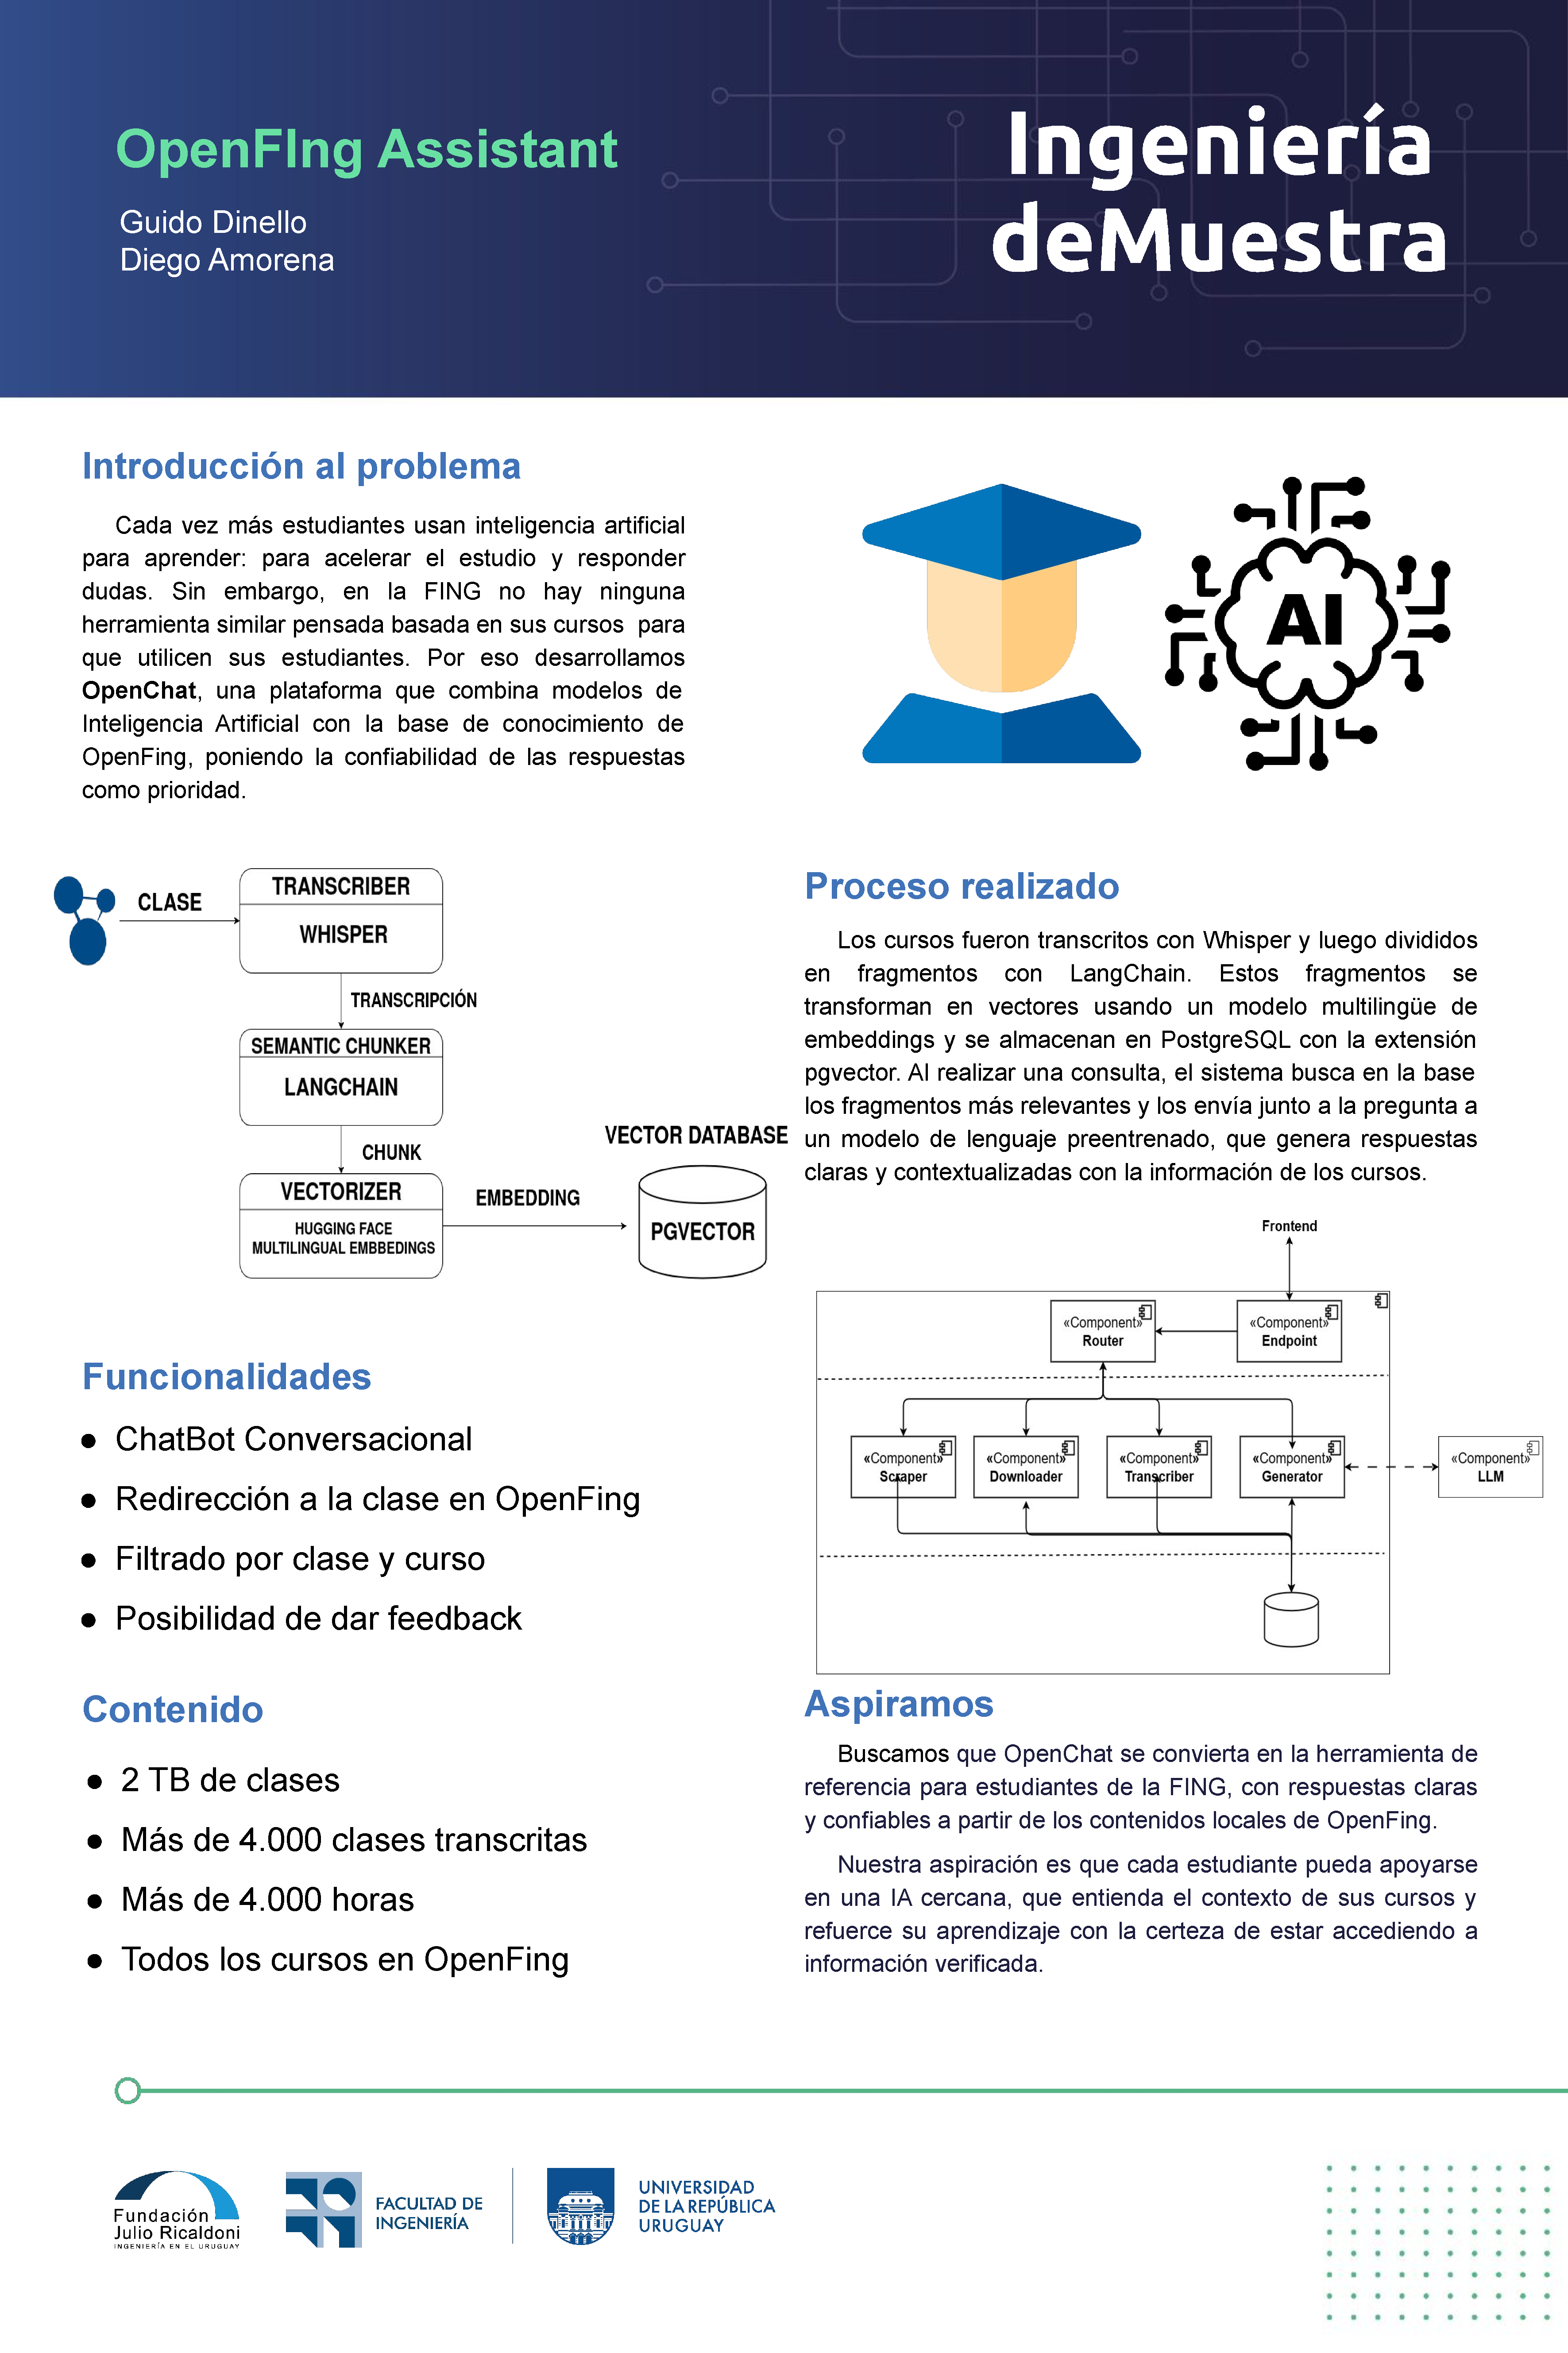
\includegraphics[width=\linewidth]{Nuestro/Otros_Documentos/Poster.pdf}
    \caption{Poster presentado. Ilustración propia.}
    \label{fig:IDM-poster}
\end{figure}